\documentclass{standalone}
\usepackage{tikz}

\begin{document}
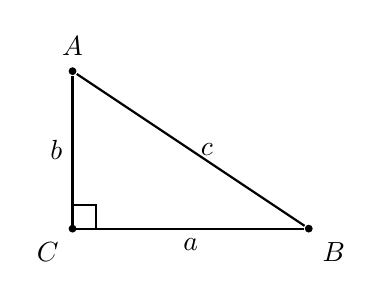
\begin{tikzpicture}[
  thick,
  trig/.style={
    circle,
    fill=black,
    inner sep=1pt,
  }
  ]
  \node (c) at (0,0) [trig,label=below left:\(C\)]{};
  \node (a) at (0,2) [trig,label=above:\(A\)]{};
  \node (b) at (3,0) [trig,label=below right:\(B\)]{};
  \draw (c) -- (a) node[midway,left] {\(b\)};
  \draw (c) -- (b) node[midway,below] {\(a\)};
  \draw (a) -- (b) node[midway,right] {\(c\)};
  % Right angle square
  \draw (c) rectangle ++(0.3,0.3);
\end{tikzpicture}
\end{document}
